%note: don't split this document up with include{...}

\section{DFAFramework}

\subsection{Klassendiagramm}
\begin{figure}[htbp] 
	\centering
	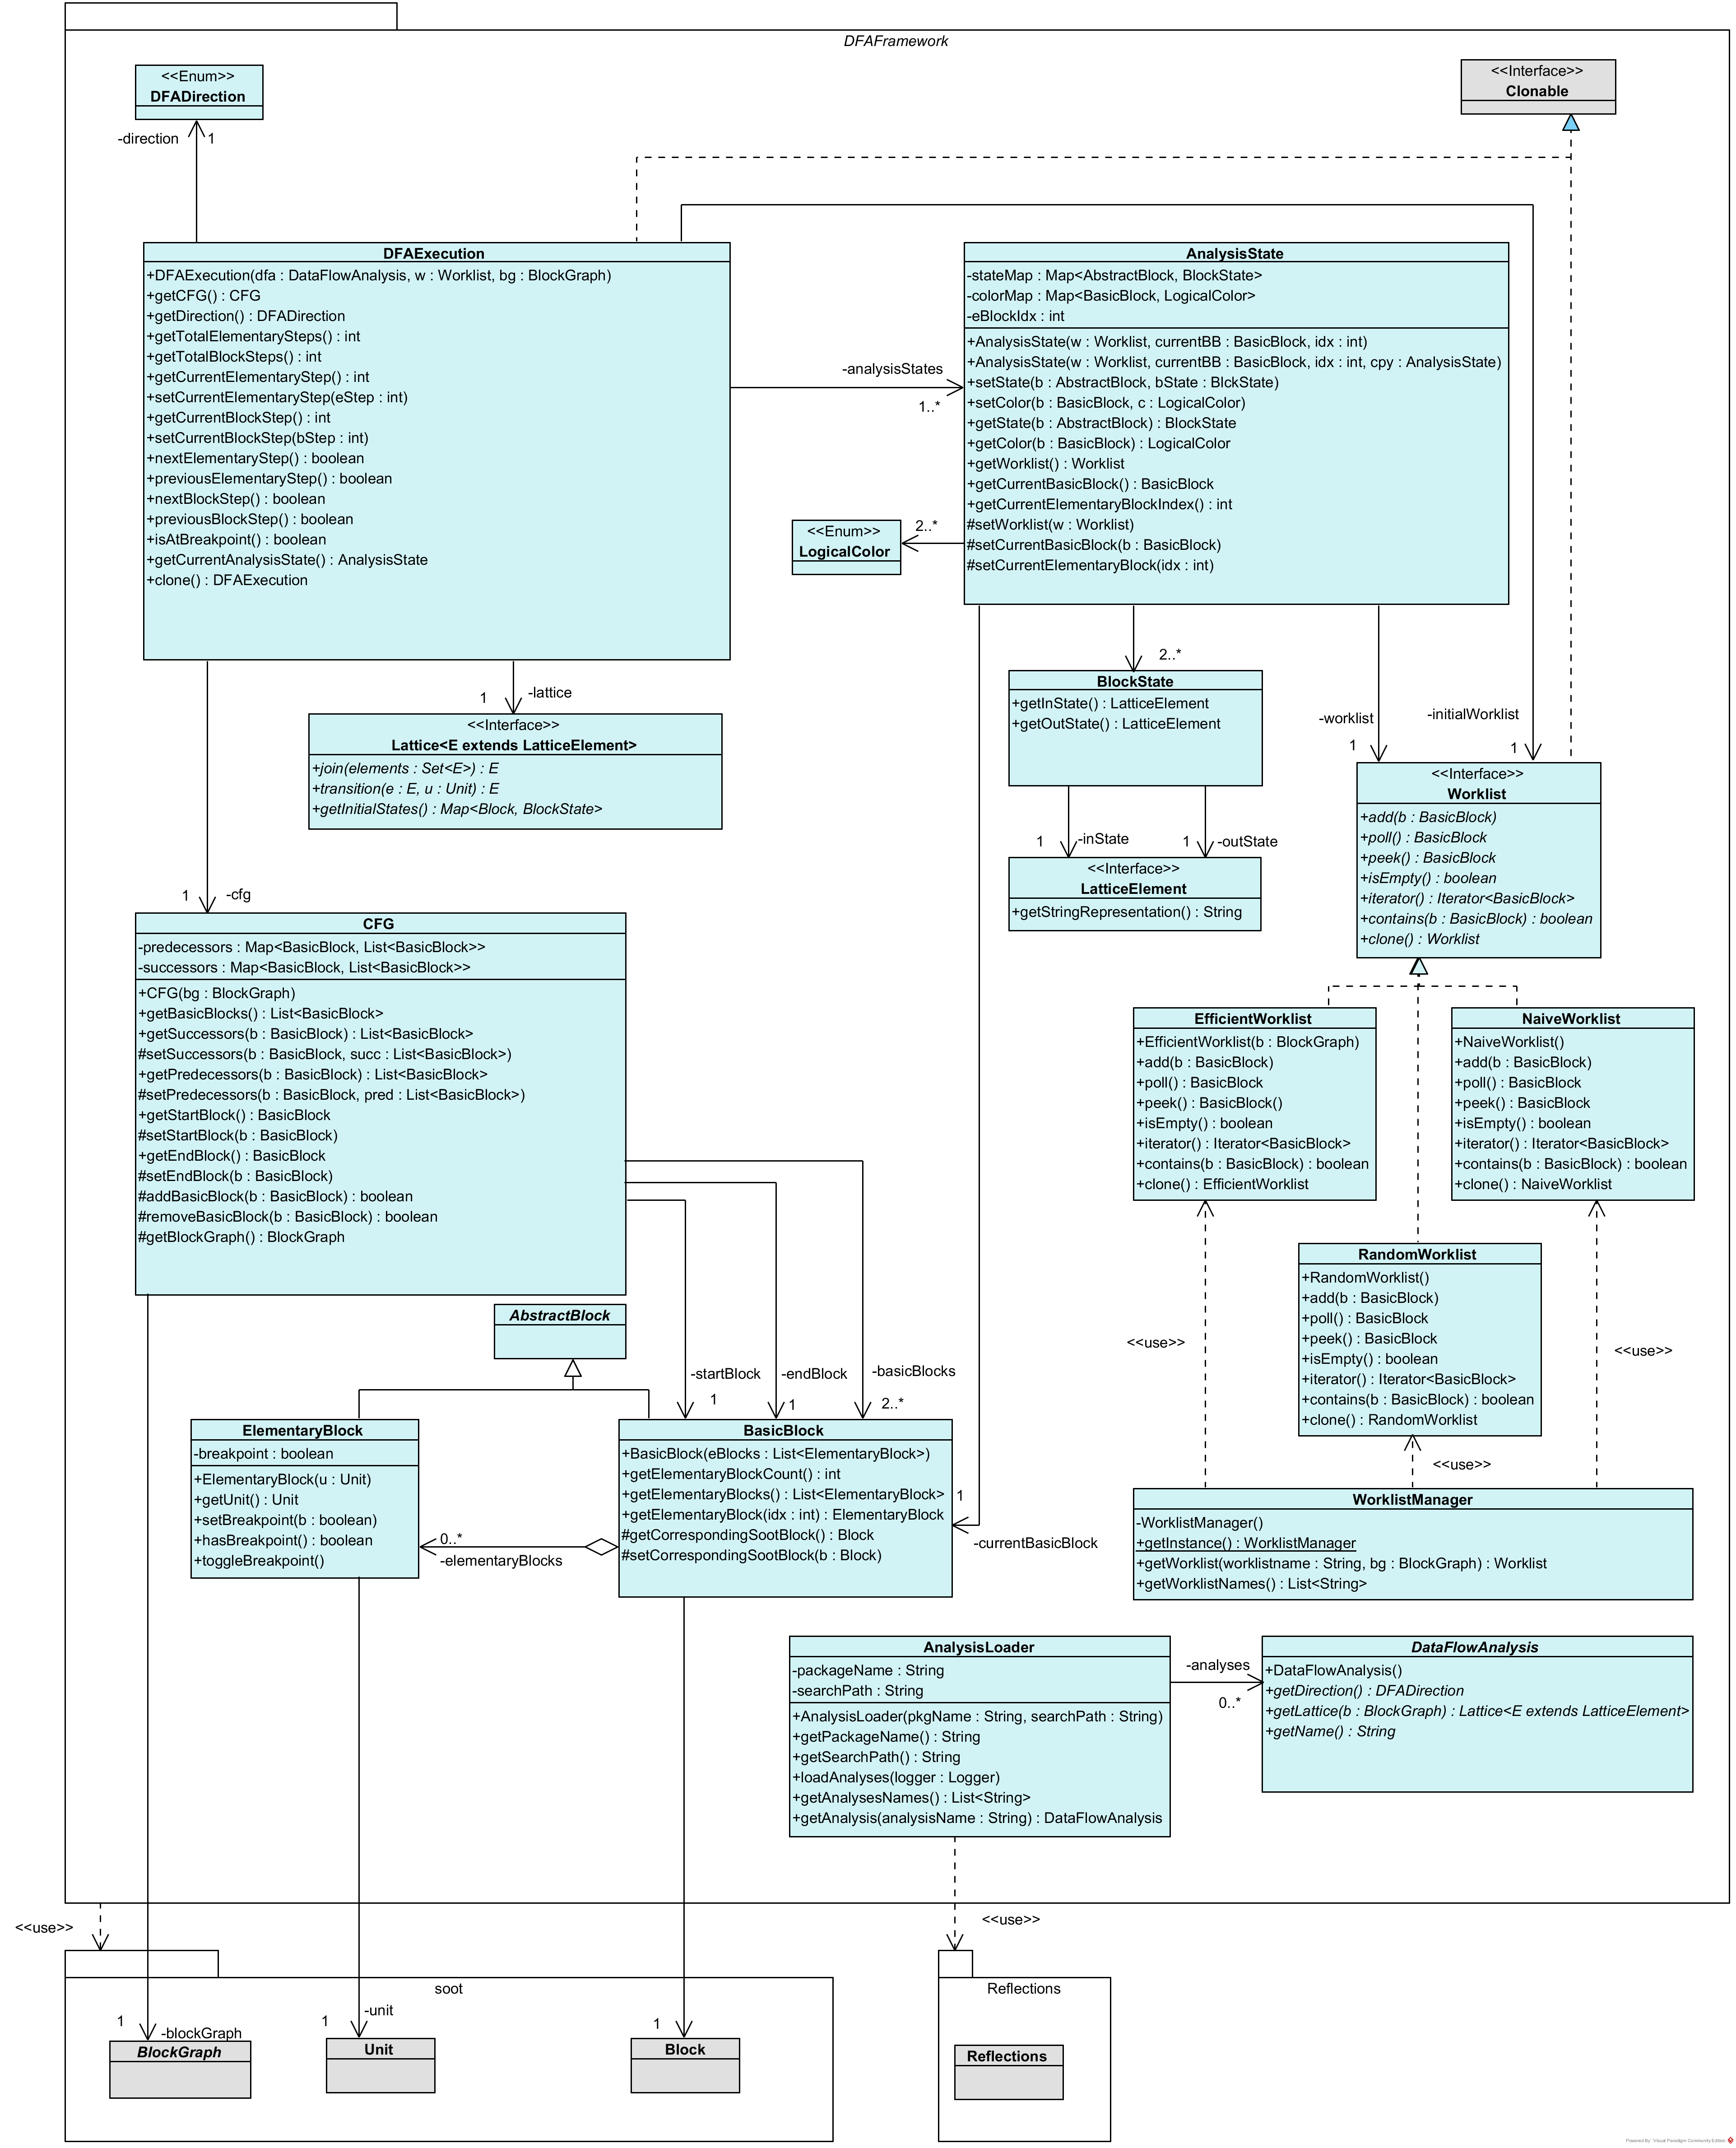
\includegraphics[width=1\textwidth]{Klassenuebersicht/DFAFramework/DFAFramework}
	\caption{Klassendiagramm des DFAFramework}
	\label{fig:DFAFreamework}
\end{figure}

%\newpage

Das DFAFramework ist für die Ausführung von Datenflussanalysen zuständig.
Weiter übernimmt das DFAFramework das Laden von Datenflussanalysen von einem festgelegten Speicherort.

Für die Ausführung von Datenflussanalysen ist die Klasse \inlinecode{DFAExecution} zentral.
Diese kann eine Datenflussanalyse für ein gegebenes \inlinecode{DataFlowAnalysis}-Objekt und einen gegebenen \inlinecode{BlockGraph} (\inlinecode{soot.toolkits.graph.BlockGraph}) vorberechnen.
Nach der Vorberechnung kann dann der aktuelle Analyseschritt mittels \inlinecode{nextElementaryStep()}, \inlinecode{previousElementaryStep()}, \inlinecode{setCurrentElementaryStep(stepNum : int)} und \inlinecode{getCurrentElementaryStep() : int} zeilenweise beliebig eingestellt bzw. abgefragt werden. 
Analog zu zeilenweisen Schritten können auch blockweise Schritte mittels \inlinecode{nextBlockStep()}, \inlinecode{previousBlockStep()}, \inlinecode{setCurrentBlockStep(step : int)} eingestellt und abgefragt werden.
Zudem kann mit \inlinecode{getCurrentAnalysisState() : AnalysisState} zu jedem Zeitpunkt der aktuelle Analysezustand erfragt werden.
Ein \inlinecode{AnalysisState} speichert dabei für jeden \inlinecode{AbstractBlock} (also sowohl für \inlinecode{ElementaryBlock}s als auch \inlinecode{BasicBlock}s) den aktuellen In- und Out-State, den aktuellen Zustand der \inlinecode{Worklist} sowie bei welchem \inlinecode{ElementaryBlock} bzw. \inlinecode{BasicBlock} sich die Analyse aktuell befindet.

Das Interface \inlinecode{Worklist} sowie die implementierenden Klassen \inlinecode{EfficientWorklist}, \inlinecode{NaiveWorklist} und \inlinecode{RandomWorklist} legen die Analysereihenfolge der einzelnen \inlinecode{BasicBlock}s fest.

Für die Implementierung konkreter Datenflussanalysen ist die Klasse \inlinecode{DataFlowAnalysis} essentiell.
Sie legt die Analyserichtung (\inlinecode{DFADirection}) sowie den Namen, unter der eine Datenflussanalyse in der GUI auftaucht, fest.
Weiter bestimmt eine \inlinecode{DataFlowAnalysis} mittels \inlinecode{getLattice(blockGraph : BlockGraph) : Lattice} den für die Analyse verwendeten Verband.
Ein \inlinecode{Lattice} realisiert den Join-Operator mittels \inlinecode{join(elements : Set<LatticeElement>) : LatticeElement}.
Weiter gibt er zu allen unterstützten Expressions eine Übergangsfunktion mittels \inlinecode{transition(in : LatticeElement, unit : soot.Unit) : LatticeElement} an.
Schließlich gibt ein \inlinecode{Lattice} zu jedem Grundblock mittels \inlinecode{getInitialStates() : Map<Block, BlockState>} einen Initialzustand an.

Ein \inlinecode{AnalysisLoader} ist für das Laden von Datenflussanalysen zuständig.
Mittels \inlinecode{loadAnalyses(logger : java.util.logging.Logger)} werden alle Unterklassen von \inlinecode{DataFlowAnalysis}, die an einem festgelegten Speicherort als .class-Dateien abgelegt sind geladen.
Die Namen der geladenen Analysen können dann mit \inlinecode{getAnalysesNames() : List<String>} abgefragt werden.
Weiter kann mit \inlinecode{getAnalysis(analysisName : String) : DataFlowAnalysis} ein \inlinecode{DataFlowAnalysis}-Objekt über seinen Namen ermittelt werden.
subsection{Klassenbeschreibung}

\newpage

\class{DFAExecution}
\todo{Class description}

\paragraph*{Attribute}
\begin{itemize}
	\item \attr{blockGraph}{BlockGraph}{private} {
	Der mit Soot aus dem durch den Benutzer eingegebenen Java-Code erstellte \inlinecode{BlockGraph}.	
	}
	\item \attr{initialWorklist}{Worklist}{private}{
	Eine \inlinecode{Worklist}, die für die Ausführung der Datenflussanalyse verwendet wird.
	}
\end{itemize}

\paragraph*{Konstruktoren} 
\begin{itemize}
	\item \ctor{DFAExecution}{dfa : AbstractDataFlowAnalysis, w : Worklist}{public}{
	Erzeugt eine \inlinecode{DFAExecution} mit folgenden Parametern:
	\begin{itemize}[topsep=-8pt] \setlength\itemsep{-12pt}
		\item eine \inlinecode{AbstractDataFlowAnalysis}, welche angibt, welche Art der Datenflussanalyse ausgeführt wird
		\item eine \inlinecode{Worklist}, die zur Ausführung der Datenflussanalyse verwendet wird
		\item ein \inlinecode{BlockGraph}, der dem kontrollflussgraphen des zu analysierenden Codes entspricht 
	\end{itemize}
	Ein \inlinecode{CFG} wird aus dem \inlinecode{BlockGraph} erstellt. 
	Alle Schritte der Datenflussanalyse	werden vorberechnet.
	}
\end{itemize}

\paragraph*{Methoden}
\begin{itemize}
	\item \method{getCFG}{CFG}{}{public}{
	Gibt den \inlinecode{CFG} zurück, auf dem die Datenflussanalyse ausgeführt wird.
	}
	\item \method{getDirection}{DFAExecution}{}{public}{
	Gibt die Richtung der Datenflussanalyse zurück.
	}
	\item \method{getTotalElementarySteps}{int}{}{public}{
	Gibt die Gesamtanzahl der Zeilenschritte in der vorberechneten Analyse zurück.
	}
	\item \method{getTotalBlockSteps}{int}{}{public}{
	Gibt die Gesamtanzahl der Blockschritte in der vorberechneten Analyse zurück.
	}
	\item \method{getCurrentElementaryStep}{int}{}{public}{
	Gibt den aktuellen Zeilenschritt zurück.
	}
	\item \method{setCurrentElementaryStep}{void}{eStep : int}{public}{
	Setzt den aktuellen Zeilenschritt auf \inlinecode{eStep}. 
	Der Zustand der Analyse springt also an den übergebenen Zeilenschritt.
	Dabei ändert sich auch der aktuelle Blockschritt konsistent zum Zeilenschritt.
	}
	\item \method{getCurrentBlockStep}{int}{}{public}{
	Gibt den aktuellen Blockschritt zurück.
	}
	\item \method{setCurrentBlockStep}{void}{bStep : int}{public}{
	Setzt den aktuellen Blockschritt auf \inlinecode{bStep}. 
	Der Zustand der Analyse springt also an die übergebene Stelle.
	Dabei ändert sich auch der aktuelle Zeilenschritt konsistent zum Blockschritt.
	}
	\item \method{nextElementaryStep}{boolean}{}{public}{
	Inkrementiert den aktuellen Zeilenschritt um eins. 
	Die Analyse springt also zur nächsten Zeile.
	Dabei ändert sich ggf. der aktuelle Blockschritt konsistent zum Zeilenschritt.
	Gibt zurück, ob das Springen zur nächsten Zeile erfolgreich war.
	}
	\item \method{previousElementaryStep}{boolean}{}{public}{
	Dekrementiert den aktuellen Zeilenschritt um eins. 
	Die Analyse springt also zur vorherigen Zeile.
	Dabei ändert sich ggf. der aktuelle Blockschritt konsistent zum Zeilenschritt.
	Gibt zurück, ob das Springen zur vorherigen Zeile erfolgreich war.
	}
	\item \method{nextBlockStep}{boolean}{}{public}{
	Inkrementiert den aktuellen Blockschritt um eins. 
	Die Analyse springt also zum nächsten Block.
	Dabei ändert sich ggf. der aktuelle Zeilenschritt konsistent zum Blockschritt.
	Gibt zurück, ob das Springen zum nächsten Block erfolgreich war.
	}
	\item \method{previousBlockStep}{boolean}{}{public}{
	Dekrementiert den aktuellen Blockschritt um eins. 
	Die Analyse springt also zum vorherigen Block.
	Dabei ändert sich ggf. der aktuelle Zeilenschritt konsistent zum Blockschritt.
	Gibt zurück, ob das Springen zum vorherigen Block erfolgreich war.
	}
	\item \method{isAtBreakpoint}{boolean}{}{public}{
	Gibt zurück, ob sich in der Zeile, in der sich die Datenflussanalyse aktuell befindet, ein Breakpoint befindet.	
	}
	\item \method{getCurrentAnalysisState}{AnalysisState}{}{public}{
	Gibt den aktuellen Zustand der Analyse zurück.	
	}
\end{itemize}

\class{CFG}
\todo{Class description}

\paragraph*{Attribute}
\begin{itemize}
	\item \attr{basicBlocks}{List<BasicBlock>}{private} {
	Liste der \inlinecode{BasicBlock}s des \inlinecode{CFG}.
	}
	\item \attr{startBlock}{BasicBlock}{private}{
	Der Startblock des \inlinecode{CFG}.
	}
	\item \attr{endBlock}{BasicBlock}{private}{
	Der Endblock des \inlinecode{CFG}.
	}
	\item \attr{predecessors}{Map<BasicBlock, List<BasicBlock>>}{private}{
	\inlinecode{Map}, die jedem \inlinecode{BasicBlock} seine Vorgänger zuordnet.
	}
	\item \attr{successors}{Map<BasicBlock, List<BasicBlock>>}{private}{
	\inlinecode{Map}, die jedem \inlinecode{BasicBlock} seine Nachfolger zuordnet.
	}
\end{itemize}

\paragraph*{Konstruktoren} 
\begin{itemize}
	\item \ctor{CFG}{blockGraph : BlockGraph}{public}{
	Erzeugt einen \inlinecode{CFG} aus einem gegebenen \inlinecode{BlockGraph}.
	}
\end{itemize}

\paragraph*{Methoden}
\begin{itemize}
	\item \method{getBasicBlocks}{List<BasicBlock>}{}{public}{
	Gibt die Liste der \inlinecode{BasicBlock}s zurück.
	}
	\item \method{getSuccessors}{List<BasicBlock>}{bBlock : BasicBlock}{public}{
	Gibt die Nachfolger des übergebenen \inlinecode{BasicBlock}s zurück.
	}	
	\item \method{setSuccessors}{void}{bBlock : BasicBlock, succ : List<BasicBlock>}{public}{
	Setzt die übergebene Liste an \inlinecode{BasicBlock}s als Nachfolger von \inlinecode{bBlock}.
	}	
	\item \method{getPredecessors}{List<BasicBlock>}{bBlock : BasicBloc}{public}{
	Gibt die Vorgänger des übergebenen \inlinecode{BasicBlock}s zurück.
	}	
	\item \method{setPredecessors}{void}{bBlock : BasicBlock, succ : List<BasicBlock>}{public}{
	Setzt die übergebene Liste an Grundblöcken als Vorgänger von \inlinecode{bBlock}.
	}	
	\item \method{getStartBlock}{BasicBlock}{}{public}{
	Gibt den Startblock des \inlinecode{CFG} zurück.
	}	
	\item \method{setStartBlock}{void}{startBlock : basicBlock}{public}{
	Setzt den übergebenen \inlinecode{BasicBlock} als Startblock des \inlinecode{CFG}.
	}
	\item \method{getEndBlock}{BasicBlock}{}{public}{
	Gibt den Endblock des \inlinecode{CFG} zurück.
	}
	\item \method{setEndBlock}{void}{endBlock : basicBlock}{public}{
	Setzt den übergebenen \inlinecode{BasicBlock} als Endblock des \inlinecode{CFG}.
	}
	\item \method{addBasicBlock}{boolean}{bBlock : basicBlock}{public}{
	Fügt den übergebenen \inlinecode{BasicBlock} zum \inlinecode{CFG} hinzu.
	Gibt zurück, ob der \inlinecode{BasicBlock} hinzugefügt werden konnte.
	}
	\item \method{removeBasicBlock}{boolean}{bBlock : basicBlock}{public}{
	Entfernt den übergebenen \inlinecode{BasicBlock} aus dem \inlinecode{CFG}.
	Gibt zurück, ob der \inlinecode{BasicBlock} entfernt werden konnte.
	}
	\item \method{getBlockGraph}{BlockGraph}{}{public}{
	Gibt den \inlinecode{BlockGraph}, auf welchem der \inlinecode{CFG} basiert, zurück.
	}
\end{itemize}

\class{AnalysisState}
\todo{Class description}

\paragraph*{Attribute}
\begin{itemize}
	\item \attr{stateMap}{Map<AbstractBlock, BlockState>}{private} {
	Eine \inlinecode{Map}, welche jedem \inlinecode{BasicBlock} einen \inlinecode{BlockState} zuordnet, welcher den aktuellen In- und Out-State des Blocks repräsentiert.
	}
	\item \attr{colorMap}{Map<BasicBlock, LogicalColor>}{private}{
	Eine \inlinecode{Map}, welche jedem \inlinecode{BasicBlock} eine \inlinecode{LogicalColor} zuordnet.
	Dabei beschreibt eine \inlinecode{LogicalColor} den Zustand eines \inlinecode{BasicBlock}s im Bezug auf die Worklist (siehe \inlinecode{LogicalColor}).
	}
	\item \attr{worklist}{Worklist}{private}{
	Die aktuelle \inlinecode{Worklist}, welche die \inlinecode{BasicBlock}s enthält, die noch zu bearbeiten sind.
	}
	\item \attr{currentBasicBlock}{BasicBlock}{private}{
	Der \inlinecode{BasicBlock}, welcher im aktuellen Analysezustand bearbeitet wird.
	}
	\item \attr{eBlockIdx}{int}{private}{
	Der Index des im aktuellen Analysezustand bearbeiteten \inlinecode{ElementaryBlock}s.
	}
\end{itemize}

\paragraph*{Konstruktoren} 
\begin{itemize}
	\item \ctor{AnalysisState}{w : Worklist, currentBB : BasicBlock, idx : int}{public}{
	Erzeugt einen \inlinecode{AnalysisState} aus
	\begin{itemize}[topsep=-8pt] \setlength\itemsep{-12pt}
		\item einer \inlinecode{Worklist}, aus welcher durch Kopieren die \inlinecode{Worklist} des erzeugten \inlinecode{AnalysisState}s erstellt wird
		\item einem neuen aktuellen \inlinecode{BasicBlock}
		\item dem Index des neuen aktuellen \inlinecode{ElementaryBlock}s 
	\end{itemize}
	}
	\item \ctor{AnalysisState}{w : Worklist, currentBB : BasicBlock, idx : int, cpy : AnalysisState}{public}{
	Erzeugt einen \inlinecode{AnalysisState}, aus
	\begin{itemize}[topsep=-8pt] \setlength\itemsep{-12pt}
		\item einer \inlinecode{Worklist}, aus welcher durch Kopieren die \inlinecode{Worklist} des erzeugten \inlinecode{AnalysisState}s erstellt wird
		\item dem neuen aktuellen \inlinecode{BasicBlock}
		\item dem neuen aktuellen Index des \inlinecode{ElementaryBlock}s
		\item einem \inlinecode{AnalysisState}, von dem das Mapping von \inlinecode{BasicBlock}s zu \inlinecode{BlockState}s übernommen wird
	\end{itemize}
	}
\end{itemize}

\paragraph*{Methoden}
\begin{itemize}
	\item \method{setState}{void}{block : AbstractBlock}{public}{
	Setzt den Zustand eines übergebenen \inlinecode{AbstractBlock}s auf den übergebenen  \inlinecode{BlockState}.	
	}
	\item \method{setColor}{void}{block : BasicBlock, c : LogicalColor}{public}{
	Setzt die \inlinecode{LogicalColor} eines übergebenen \inlinecode{BasicBlock}s.
	}
	\item \method{getState}{BlockState}{block : AbstractBlock}{public}{
	Gibt den aktuellen \inlinecode{BlockState} des übergebenen \inlinecode{AbstractBlock}s zurück.
	}
	\item \method{getColor}{LogicalColor}{block : BasicBlock}{public}{
	Gibt die aktuelle \inlinecode{LogicalColor} des übergebenen \inlinecode{BasicBlock}s zurück.
	}
	\item \method{getWorklist}{Worklist}{}{public}{
	Gibt die \inlinecode{Worklist} in diesem \inlinecode{AnalysisState} zurück.
	}
	\item \method{getCurrentBasicBlock}{BasicBlock}{}{public}{
	Gibt den aktuellen \inlinecode{BasicBlock} zurück.
	}
	\item \method{getCurrentElementaryBlock}{ElementaryBlock}{}{public}{
	Gibt den aktuellen \inlinecode{ElementaryBlock} zurück.
	}
	\item \method{getCurrentElementaryBlockIndex}{int}{}{public}{
	Gibt den Index der des aktuellen \inlinecode{ElementaryBlock}s zurück.
	}
	\item \method{setWorklist}{void}{worklist : Worklist}{protected}{
	Setzt die übergebene \inlinecode{Worklist} als aktuelle \inlinecode{Worklist} dieses \inlinecode{AnalysisState}s.
	}
	\item \method{setCurrentBasicBlock}{void}{bBlock : basicBlock}{protected}{
	Setzt den übergebenen \inlinecode{BasicBlock} als den aktuellen \inlinecode{BasicBlock}.
	}
	\item \method{setCurrentElementaryBlock}{void}{idx : int}{protected}{
	Setzt den übergeben Index als Index des aktuellen \inlinecode{ElementaryBlock}s.
	}
\end{itemize}

%\item \method{name}{ret}{param : type}{public}{
%	
%}
